\documentclass[11pt]{article}

% set these commands
\newcommand{\course}{CSCI 534}
\newcommand{\proj}{Homework 01}
\newcommand{\dueDate}{1-28-2021}
\newcommand{\name}{Nathan Stouffer}

\usepackage{../macros}

\newcommand{\pareto}[1]{\rm{Pareto}(#1)}
\newcommand{\conv}[1]{\rm{conv}(#1)}



\begin{document}

\coverpage{02}

\newpage
\section*{Problem 1}

Assume you are given a planar subdivision with $n$ faces in a DCEL. (You may
assume that the planar subdivision does not contain any holes, i.e., there are
no nested faces.) Give pseudo-code for an algorithms that given a vertex $v$ of
the DCEL, outputs all neighbors of $v$. \\\\
\answer
Here is a quick prose description of the algorithm and the pseudo-code is given below in Algorithm \ref{alg:neighbors}.
We are given a vertex $v$ in a DCEL and we want to compute the neighbors of $v$.
We start with an edge pointing at $v$ and then move clockwise around the edges pointing at $v$, adding the origins.

\begin{algorithm}
\caption{Computing the neighbors of $v$}
\label{alg:neighbors}
    \begin{algorithmic}[1]
    \Function{Neighbors}{$v$}
        \State nbhd $\gets $ empty stack
        \State $e \gets v$.inc\_edge.twin
        \State nbhd.push($e$.orig)
        \State $\overline{e} \gets$ $e$.next.twin
        \While{$e \neq \overline{e}$}
            \State nbhd.push($\overline{e}$.orig)
            \State $\overline{e} \gets \overline{e}$.next.twin
        \EndWhile
        \State \Return nbhd
    \EndFunction
    \end{algorithmic}
\end{algorithm}

Now we will present a proof of correctness.
At the end of the $i^{th}$ iteration of the while loop, denote the value of $\overline{e}$ as $\overline{e}_i$.
We then have the following loop invariant: $\overline{e}_{i}$ is the clockwise edge following $\overline{e}_{i-1}$ around $v$ (that points at $v$).
The loop invariant is preserved since we use the properties of edges in a DCEL to set $\overline{e}_{i}$ to $\overline{e}_{i-1}$.next.twin, the next clockwise edge around $v$ that points at $v$.
We repeat until we return to the original edge.
Then a vertex $w$ is a neighbor to $v$ if and only if there is an edge from $w \to v$ (symmetry implies $v \to w$ exists).
Since we process all edges pointing to $v$ and we add each source, we have every neighbor of $v$.
Thus the algorithm is correct.
We can quickly derive the runtime.
We loop over each neighbor of $v$ exactly once so we can bound iterations with the number of vertices $n$.
Therefore the run time is $O(n)$.

\begin{figure}[h]
   \centering
   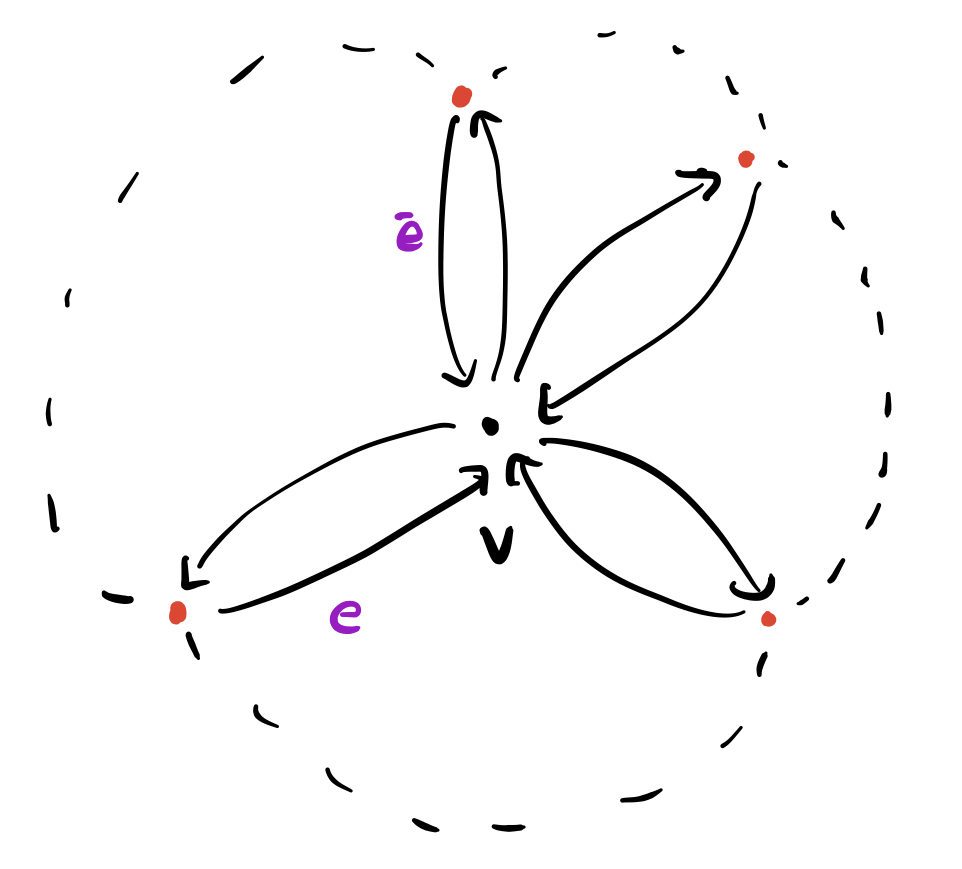
\includegraphics[width=0.3\textwidth]{nbhd}
   \caption{Neighbors of $v$}
   \label{fig:neighbors}
\end{figure}

\newpage
\section*{Problem 2}

Assume you are given a planar subdivision of $O(n)$ size in a DCEL. (You may
assume that the planar subdivision does not contain any holes, i.e., there are
no nested faces.) Describe an algorithm that for a given point $p$ in the plane
finds the face in the subdivision that contains it. Your algorithm should run in
$O(n)$ time. You do not have to write pseudo-code, but please make clear what
DCEL operations you are using. Also please make sure the analysis is detailed
enough to justify the $O(n)$ runtime clearly. \\\\
\answer
Here is a quick description of our algorithm.
We gain some inspiration from Gauss' Law in physics.
At the highest level, we iterate over each face in the DCEL and check if the query point is in the face.
We know a point is in a face if and only if a ray originating at the point passes through the boundary an odd number of times.
We know the exact boundary of the face by looping over each edge on the face.
We also only consider the edges that have a pointer to this face (we ignore the twin).

\begin{algorithm}
\caption{Find the face where $p$ resides}
    \label{alg:findface}
    \begin{algorithmic}[1]
    \Function{FindFace}{DCEL, $p$}
        \For{face in DCEL}
            \State cnt $\gets$ \textsc{CountIntersections}(face, $p$)
            \If{cnt $\equiv 1 \mod 2$}
                \State \Return face
            \EndIf
        \EndFor
    \EndFunction
    \end{algorithmic}

    \begin{algorithmic}[1]
    \Function{CountIntersections}{face, $p$}
        \State cntr $\gets 0$
        \State $h \gets$ horizontal line passing through $p_y$
        \For{each edge $e$ incident to face}
            \State $l \gets$ line passing through the edge $e$
            \State $x \gets$ $x$ coordinate of the intersection between $h$ and $l$
            \If{$x \geq p_x$ and $x$ is between $e$.orig$_x$ and $e$.twin.orig$_x$}
                \State cntr $\gets$ cntr + 1
            \EndIf
        \EndFor
        \State \Return cntr
    \EndFunction
    \end{algorithmic}
\end{algorithm}

We claim the run time of this algorithm is $O(n)$.
On slack, we idenitified that $n$ represents the number of vertices in the DCEL.
However, it was also noted that the number of edges in an embedded planar graph is $O(n)$.
In the very worst case, our algorithm would have to process every edge once.
An edge cannot be processed more than once because each edge is associated with only one face (we are ignoring twins).
Therefore our run time is $O(n)$.

Now we must show correctness.
We assume that no vertices in the DCEL share $x$ coordinates and that the point $p$ is entirely inside a face in the DCEL (not a vertex or on an edge).
We define the parity of a ray $r$ with respect to a polygon $P$ to be the parity of the number of times $r$ crosses the boundary of $P$.
Our algorithm relies on the statement a point $p$ is inside a polygon $P$ if and only if every ray originating at $p$ has odd parity with respect to $P$.
We take for granted that all rays originating at $p$ have the same parity with respect to $P$.
Figure \ref{fig:crossings} is quite helpful for illustrating the ideas presented in the following proof.

\begin{figure}[h]
   \centering
   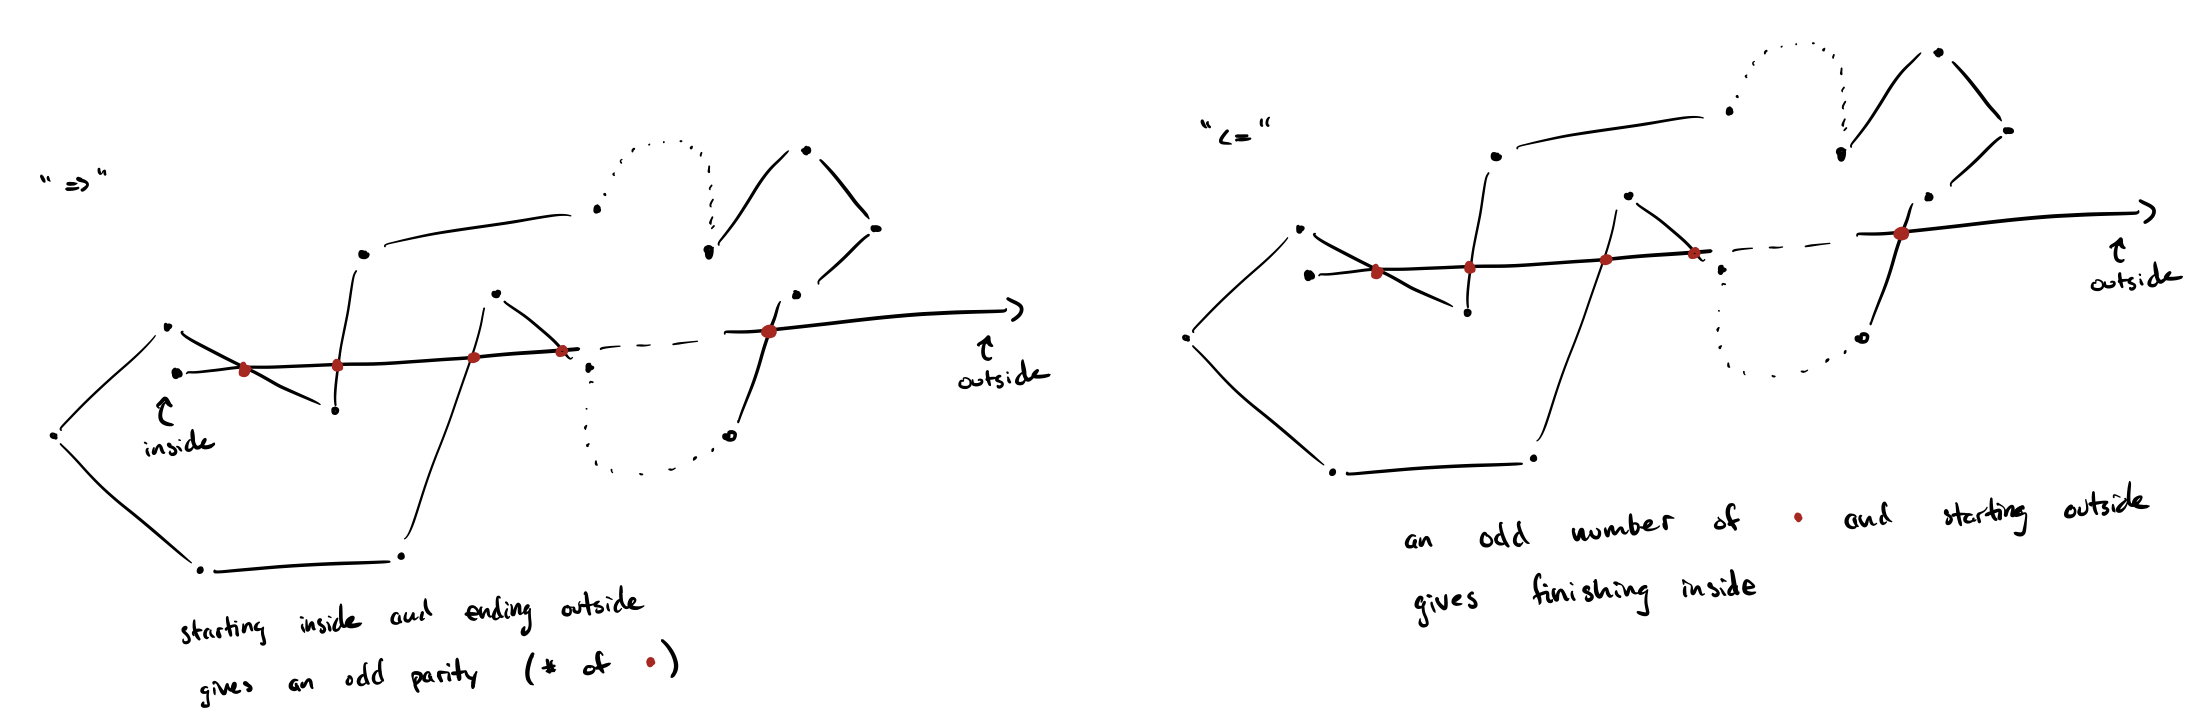
\includegraphics[width=0.95\textwidth]{crossings}
   \caption{Ray parity}
   \label{fig:crossings}
\end{figure}

Going to the left, suppose $p$ is inside the polygon $P$.
Without loss of generality, choose a ray $r$ originating at $p$.
Since $P$ is bounded but $r$ is not, we know $r$ is outside $P$ at ``infinity.''
Every crossing is a swap from inside $P$ to outside $P$ (or vice versa).
We begin inside $P$ and end outside $P$ so there must be an odd number of crossings which means that $r$ has odd parity.
By arbitrariness of $r$, every ray originating at $p$ has odd parity.
Now going to the right, suppose every ray originating at $p$ as odd parity with respect to $P$.
Without loss of generality, pick a ray $r$.
At ``infinity,'' we know $r$ is outside $P$.
We begin outside and make an odd number of swaps, so we must end up inside $P$.

Therefore, for every face, we only need to pick a ray and compute the parity of the number of crossings.
This is exactly what our algorithm does for the ray originating at $p$ and going in the positive $x$ direction!

\newpage
\section*{Problem 3}

Assume you are given a collection of $n$ circles $\{C_1 , \ldots , C_n \}$ in
$\R^2$, where circle $C_i$ is presented as its center point $q_i = (x_i, y_i)$
and radius $r_i > 0$. Present an $O(n \log n)$ time algorithm that determines
whether any two circles intersect. Note that one circle may be nested within
another without intersecting. Your algorithm should either output
that there is no intersection, or that there is at least one intersection, and
if so it will output the indices of $i$ and $j$ of two circles $C_i$ and $C_j$
that intersect. Irrespective of the number of intersecting pairs, it need only
output one intersecting pair. \\\\
\answer
First we give a description of our algorithm.
We landed on an algorithm that is very similar to the algorithm presented in class for for computing the number of intersections in a set of straigt line segments.
We will sweep from left to right across the circles, making decisions at event points.
We define a left point on a circle to be the point with the smallest $x$ coordinate of the circle (see Figure \ref{fig:lrpoints}).
For the circle $C_i$ this is the point $(x_i - r_i, y_i) \in \R ^2$ (similarly, we have a right point).
Left points and right points make up the event types.
Because we are given the circles, we know all the left and right points prior to beginning the sweep.
This means that we do not need a fancy data structure to store the event points, we can just sort them into a queue and pop them as needed.

\begin{figure}[h]
   \centering
   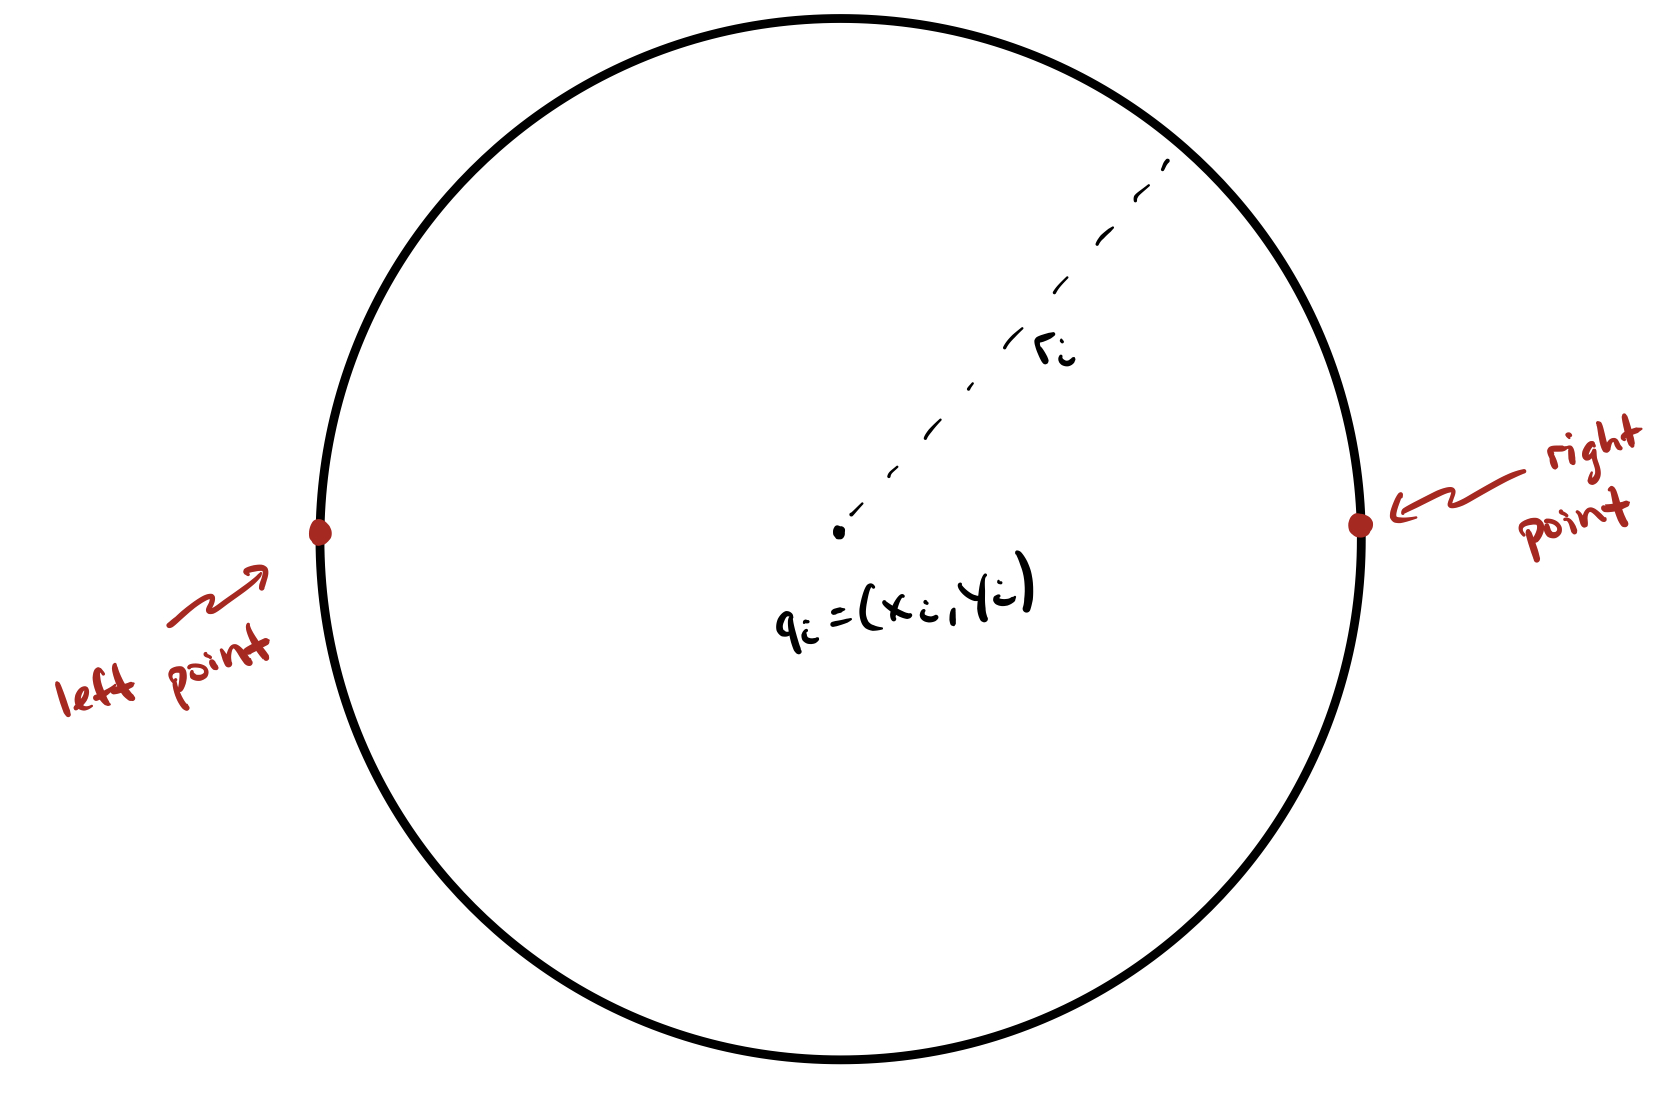
\includegraphics[width=0.65\textwidth]{lrpoints}
   \caption{Depicting the left and right points of a circle}
   \label{fig:lrpoints}
\end{figure}

The actual items in the event queue will be a triple $(p, i, type)$ where $p = (p_x, p_y) \in \R ^2$, $i$ is the index of the circle $C_i$ associated with $p$ (since $p$ is a left or right point), and $type$ denotes whether the point is a left or right point.
The key for sorting is the value of $p_x \in \R$ and we sort the list from least to greatest.
Now let's discuss the sweep line.
Just as in the segment intersection, we will store the items in an ordered dictionary.
What items will we be storing?
Instead of storing the actual circles, we will split each circle into two semi-circles and store the functions that represent them (see Figure \ref{fig:tbfunctions}).
For a circle $C_i$ represented as $q_i = (x_i, y_i)$ and $r_i > 0$, these two functions will be
$$ f_i^t (x) = y_i + \sqrt{r_i^2 - (x - x_i)^2} \hspace{2em} f_i^b (x) = y_i - \sqrt{r_i^2 - (x - x_i)^2} $$
Then we will store both pairs $(f_i^t, i)$ and $(f_i^b, i)$ in the ordered dictionary accoriding to their $y$ value at time $x$ (the time the sweep line is at).
Note that the ordered dictionary gives us the operations $search,\, delete,$ and $insert$ in $O(\log k)$ time where $k$ is the number of items in the dictionary.

\begin{figure}[h]
   \centering
   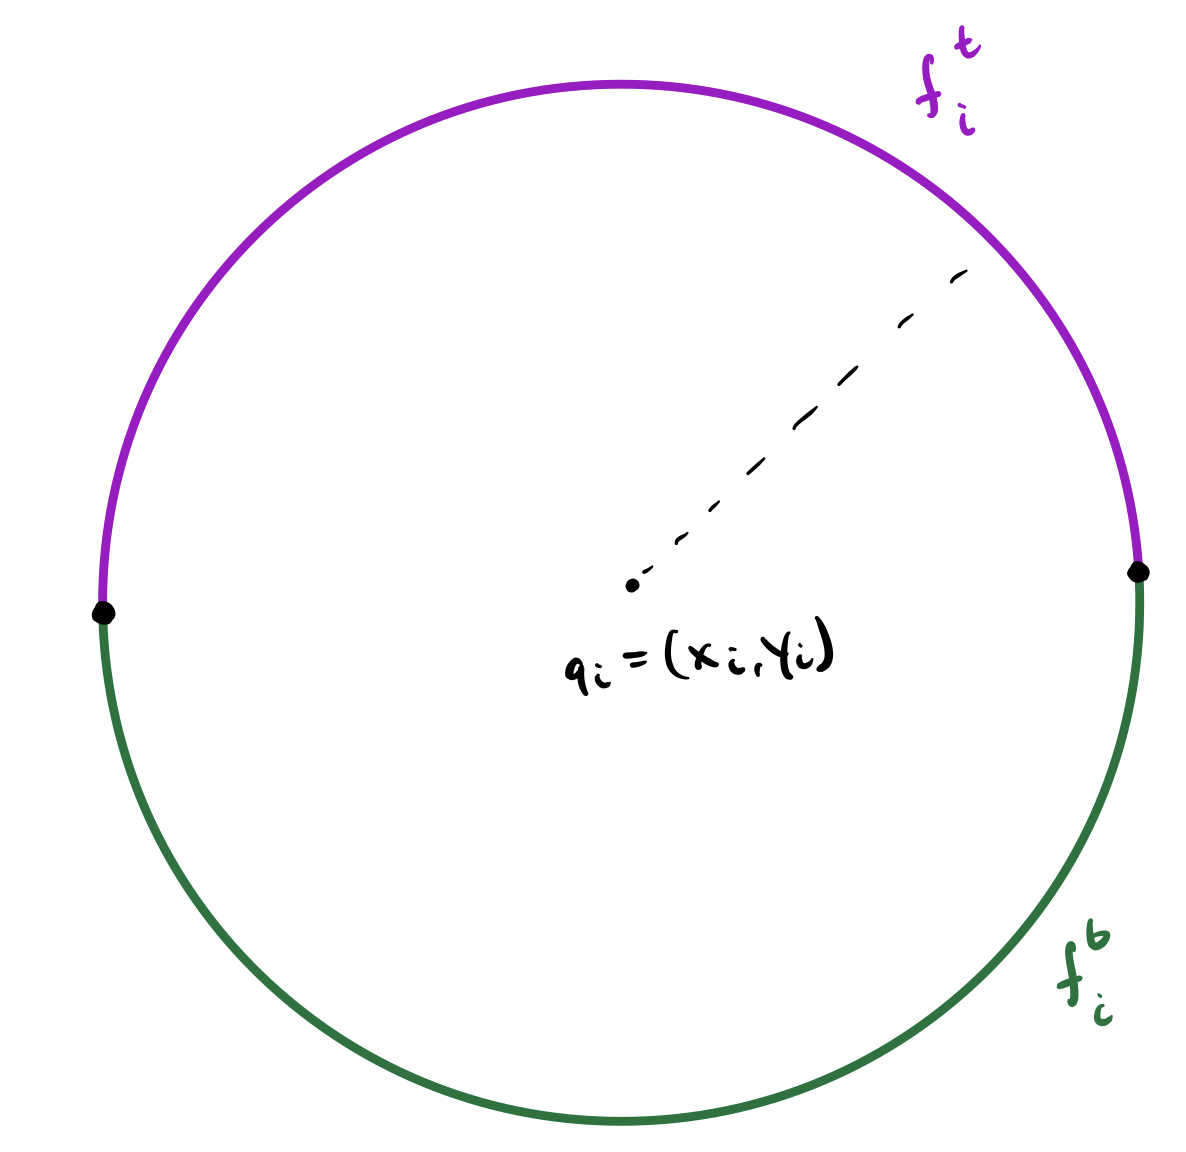
\includegraphics[width=0.5\textwidth]{tbfunctions}
   \caption{Depicting the top and bottom functions of a circle}
   \label{fig:tbfunctions}
\end{figure}

\noindent Now that we have set up the items that we will be working with, we can describe the algorithm.
\begin{enumerate}
    \item Sort events according to $p_x$, the $x$ coordinate of the point
    \item Pop event off the queue
    \item If the event is a left point, insert $(f_i^t, i)$ and $(f_i^b, i)$ into the ordered dictionary (with the top above the bottom) and check for intersections with adjacent items (ignoring each other).
    If there is an intersection, return the indices of the relevant circles.
    \item If the event is a right point, delete $(f_i^t, i)$ and $(f_i^b, i)$ from the ordered dictionary and check for intersections of the items that just became adjacent on the sweep line (the items above/below the ones just deleted).
    If there is an intersection, return the indices of the relevant circles.
    \item If the queue is empty, return NO INTERSECIONS.
    Otherwise go to line 2.
\end{enumerate}

\noindent We now show that our algorithm runs in $O(n \log n)$ time where $n$ is the number of circles.
Step 1 is the sorting of $2n$ items.
This takes $O(n \log n)$ time.
We claim one iteration of the loop beginning at Step 2 takes $O(\log n)$ time.
We perform a constant number of ordered dictionary operations, each of which take $O(\log k)$ time (where $k$ is the number of items in the dictionary).
The only bound we can place on $k$ is that it must be less than $2n$ (2 functions for each circle) so we really have $O(\log n)$.
Then there is a constant number of intersection tests which each take constant time, which leaves us with $O(\log n)$ for one iteration of the loop.
Step 2 runs at most $2n$ times (for the $2n$ events) so the loop runs in $O(n \log n)$ time.
Therefore, the whole algorithm takes $O(n \log n)$ time.

Finally, we prove that the algorithm is correct.
We assume that there is no intersection at a left or right point (this also implies that no two circles are equal).
We also assume that no 3 circles intersect at the same point.
Our proof of correctness relies on a lemma very similar to the line segment intersection.

{\bf Lemma: }
We claim that for functions $f_1, f_2$ that intersect at $a = (a_x, a_y) \in \R ^2$, the items corresponding to $f_1$ and $f_2$ are adjacent on the sweep line directly before intersecting.
Here is a proof.
We assumed that no three functions intersect at the same point, so there must be some vertical line $l$ at $x = a_x - \epsilon$ ($\epsilon > 0$) such that $f_1$ and $f_2$ are adjacent on $l$.
Now consider the event $e$ with the largest $x$ coordinate less than $a_x$.
Let $b = (b_x, b_y) \in \R ^2$ be the point where $e$ occurs.
We know that there are no events between $b_x$ and $a_x$ so the order on the sweep line remains unchanged.
Therefore, the items associated with $f_1$ and $f_2$ must be adjacent on the sweep line at event $e$.

Our algorithm merely runs through all the event points and checks if adjacent members of the sweep line intersect when they appear.
Therefore, if an intersection exists, we must find it.
If no intersections exist, we will process all the circle and return that no intersection exists.
This proves the correctness of our algorithm.

\newpage
\section*{Problem 4}

I have had a few people ask about drawings and making figures.  One tool that I
like to use is Ipe (written by Otfried Cheong).  Ipe allows you to draw content
on layers and show and hide the different layers.  Layers are very helpful if,
for example you want to draw a point set and then show how some data structures
in an algorithm change as you sweep across the point set.
Other vector graphics tools such asIllustrator and Inkscape are also quite good.

Setup Ipe \url{http://ipe.otfried.org/}, Illustrator, or Inkscape
(or another vector graphics tool)
to create 3 images of the state of the sweep line algorithm
described in problem 3.

% \section*{Tips and Acknowledgements}
%
% For drawing pictures with Ipe, check out the layer pallet (in the bottom
% left hand corner).  It is very helpful for creating algorithm animations.
%
% {\bf Acknowledgements:} Homework problems adapted from assignments of David
% Mount and Carola Wenk.

\end{document}
